%%%%%%%%%%%%%%%%%%%%%%%%%%%%%%%%%%%%%%%%%
% Vertical Line Title Page 
% LaTeX Template
% Version 1.0 (27/12/12)
%
% This template has been downloaded from:
% http://www.LaTeXTemplates.com
%
% Original author:
% Peter Wilson (herries.press@earthlink.net)
%
% License:
% CC BY-NC-SA 3.0 (http://creativecommons.org/licenses/by-nc-sa/3.0/)
% 
% Instructions for using this template:
% This title page compiles as is. If you wish to include this title page in 
% another document, you will need to copy everything before 
% \begin{document} into the preamble of your document. The title page is
% then included using \titleGM within your document.
%
%%%%%%%%%%%%%%%%%%%%%%%%%%%%%%%%%%%%%%%%%

%----------------------------------------------------------------------------------------
%	PACKAGES AND OTHER DOCUMENT CONFIGURATIONS
%----------------------------------------------------------------------------------------

\documentclass{report}

\usepackage{cite,graphicx}
\usepackage[chapter]{algorithm}
\usepackage{url,float}
\usepackage{hyperref}
\usepackage{uithesis}
\usepackage{listings}
\usepackage[nodayofweek,level]{datetime}
\usepackage[bahasai]{babel}
\selectlanguage{bahasai}
\renewcommand{\bibname}{Daftar Referensi}
\renewcommand{\contentsname}{Daftar Isi}
\renewcommand{\listfigurename}{Daftar Gambar}
\renewcommand{\listtablename}{Daftar Tabel}
\renewcommand\lstlistingname{Program}
\renewcommand\lstlistlistingname{Daftar Program}
%\def\lstlistingautorefname{Program.}
\renewcommand{\chaptername}{BAB}
\renewcommand{\figurename}{\bo{Gambar}}
\renewcommand{\tablename}{\bo{Tabel}}
\Var{\kataPengantar}{Kata Pengantar}
%
% Hyphenation untuk Indonesia 
%
% @author  Andreas Febrian
% @version 1.00
% 
% Tambahkan cara pemenggalan kata-kata yang salah dipenggal secara otomatis 
% oleh LaTeX. Jika kata tersebut dapat dipenggal dengan benar, maka tidak 
% perlu ditambahkan dalam berkas ini. Tanda pemenggalan kata menggunakan 
% tanda '-'; contoh:
% menarik
%   --> pemenggalan: me-na-rik
%

\hyphenation{
    % alphabhet A
    a-na-li-sa a-tur 
    a-pli-ka-si 
    % alphabhet B
    ba-ngun-an 
    be-be-ra-pa 
    ber-ge-rak
    ber-ke-lan-jut-an 
    ber-pe-nga-ruh 
    ber-o-pe-ra-si
    % alphabhet C
    ca-ri cri-ti-cal
    % alphabhet D
    di-sim-pan di-pim-pin de-ngan da-e-rah di-ba-ngun da-pat di-nya-ta-kan 
    di-sim-bol-kan di-pi-lih di-li-hat de-fi-ni-si
    di-mo-del-kan di-te-rap-kan
    di-ha-rap-kan
    di-e-va-lu-a-si
    di-su-sun
    di-sa-ji-kan
    % alphabhet E
    e-ner-gi eks-klu-sif
    % alphabhet F
    fa-si-li-tas
    % alphabhet G
    ga-bung-an ge-rak
    % alphabhet H
    ha-lang-an
    % alphabhet I
    % alphabhet J
    % alphabhet K
    ke-hi-lang-an
    ku-ning 
    kua-li-tas ka-me-ra ke-mung-kin-an ke-se-pa-ham-an
    % alphabhet L
    ling-kung-an
    % alphabhet M
    me-ne-ngah
    meng-a-tas-i me-mung-kin-kan me-nge-na-i me-ngi-rim-kan 
    meng-u-bah meng-a-dap-ta-si me-nya-ta-kan mo-di-fi-ka-si
    meng-a-tur
    meng-a-la-mi
    me-re-pre-sen-ta-si-kan
    men-da-pat-kan
    me-nun-juk-kan
    % alphabhet N
    nya-ta non-eks-klu-sif nu-klir
    % alphabhet O
    o-pe-ra-si
    % alphabhet P
	pe-nye-rap-an 
	pe-ngon-trol
    pe-mo-del-an
    pe-ran  pe-ran-an-nya
    pem-ba-ngun-an pre-si-den pe-me-rin-tah prio-ri-tas peng-am-bil-an 
    peng-ga-bung-an pe-nga-was-an pe-ngem-bang-an 
    pe-nga-ruh pa-ra-lel-is-me per-hi-tung-an per-ma-sa-lah-an 
    pen-ca-ri-an peng-struk-tur-an
    per-siap-an pa-ra-me-ter
    pa-sang-an
    % alphabhet Q
    % alphabhet R
    ran-cang-an
    % alphabhet S
    si-mu-la-si sa-ngat
    % alphabhet T
    te-ngah
    ter-da-pat
    % alphabhet U
    % alphabhet V
    % alphabhet W
    % alphabhet X
    % alphabhet Y
    % alphabhet Z
    % special
}


%----------------------------------------------------------------------------------------
%	TITLE PAGE
%----------------------------------------------------------------------------------------

\newcommand*{\titleGM}{\begingroup % Create the command for including the title page in the document
\hbox{ % Horizontal box
\hspace*{0.2\textwidth} % Whitespace to the left of the title page
\rule{1pt}{\textheight} % Vertical line
\hspace*{0.05\textwidth} % Whitespace between the vertical line and title page text
\parbox[b]{0.75\textwidth}{ % Paragraph box which restricts text to less than the width of the page

{\noindent\Huge\bfseries Struktur Data }\\[2\baselineskip] % Title
{\large \textit{Diktat kuliah}}\\[4\baselineskip] % Tagline or further description
{\large \textsc{Dr. Arya Adhyaksa Waskita}} % Author name

\vspace{0.5\textheight} % Whitespace between the title block and the publisher
\begin{figure}[H]

\includegraphics[scale=.2]{pics/logo.png}
\end{figure}
STMIK Eresha - 2017
%Powered by \LaTex

%{\noindent The Publisher \plogo}\\[\baselineskip] % Publisher and logo
}}
\endgroup}

%----------------------------------------------------------------------------------------
%	BLANK DOCUMENT
%----------------------------------------------------------------------------------------

\begin{document}

%\addChapter{\kataPengantar}


\pagestyle{empty} % Removes page numbers

\titleGM % This command includes the title page
\pagenumbering{roman}
\setcounter{page}{0}
\tableofcontents
\listoffigures
\addChapter{Daftar Program}
\lstlistoflistings
\addChapter{\kataPengantar}
%-----------------------------------------------------------------------------%
\chapter*{Kata Pengantar}
%-----------------------------------------------------------------------------%
Diktat kuliah struktur data diperuntukkan bagi peserta mata kuliah struktur data STMIK Eresha semester II. Diktat ini menggunakan buku \cite{adam2001data,group2005data} sebagai acuan utama. Dilengkapi juga acuan tambahan dari berbagai sumber online yang sesuai.

\vspace*{0.1cm}
\begin{flushright}
\selectlanguage{bahasai}
Serpong, \today\\[0.1cm]
\vspace*{1cm}
Dr. Arya Adhyaksa Waskita

\end{flushright}


\pagenumbering{arabic}
\chapter{Pendahuluan}
Memanfaatkan komputer dalam menyelesaikan suatu masalah menuntut pengetahuan tentang transformasi masalah tersebut agar dapat diselesaikan dengan komputer. Materi struktur data digunakan untuk memahami transfromasi data yang terlibat dalam suatu masalah serta operasi yang berlaku pada data sehingga dapat diselesaikan dengan komputer. Transformasi tersebut tentang bagaimana data diorganisasikan, dikendalikan serta struktur yang harus dirancang dan diterapkan. Targetnya adalah sebuah solusi yang sederhana dan efisien.

\section{Representasi data}
Dalam komputer, data dan instruksi dinyatakan dalam bentuk biner, berupa susunan angka $0$ dan $1$ dengan arti tertentu. Susunan 8 \texttt{bit} biner disebut dengan \texttt{byte} digunakan untuk merepresentasikan karakter. Sedangkan kumpulan karakter akan menjadi string. Ilustrasinya ditunjukkan pada Gambar \ref{fig:dataRep}.

\begin{figure}[H]
\centering
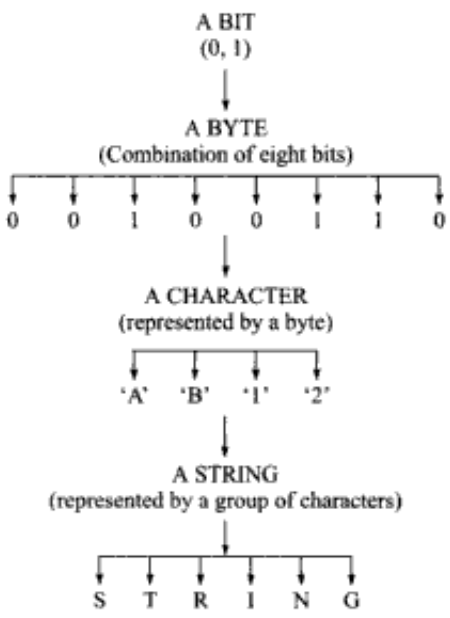
\includegraphics[scale=.45]{pics/dataRepresentation.png}
\caption{Representasi data dalam komputer}
\label{fig:dataRep}
\end{figure}

Acuan dalam merepresentasikan data ke dalam sistem biner antara adalah ASCII (\textit{American Standard Code for Information Interchange}) dan BCD (\textit{binary-coded decimal}). Dan setiap bahasa pemrograman telah mendefinisikan representasi untuk perintah dan data yang digunakannya seperti ilustrasi pada Gambar \ref{fig:dataRep}. Setiap jenis data memiliki skema representasi yang berbeda. Representasi data integer dilakukan menggunakan 8 bit (1 byte) biner. Misalnya, $27$ dinyatakan dalam bilangan biner sebagai $00011011$. Sementara untuk menyatakan bilangan negatifnya, dapat dilakukan dengan dua pendekatan. Yang pertama adalah melakukan operasi komplemen pada setiap bit biner, yaitu setiap bit $0$ diubah menjadi $1$, sedangkan bit $1$ menjadi $0$. Dengan demikian, angka $-27$ jika dinyatakan dalam biner dengan operasi komplemen menjadi $11100100$. Sedangkan representasi yang kedua adalah menambahkan angka $1$ pada hasil operasi komplemen pertama. Sehingga angka $-27$ dapat dinyatakan dalam bilangan biner dengan skenario kedua sebagai $11100101$.

Selan itu, bilangan desimal dapat juga dinyatakan dalam bilangan biner dengan terlebih dahulu memisahkan bagian bilangan bulat (mantissa) dengan bagian pangkat (eksponen)nya. Sebagai contoh, bilangan $209.52$ dapat dinyatakan sebagai $20952.10^{-2}$ dalam bilangan basis $10$. $20952$ adalah bagian mantissa, sedangkan $-2$ adalah bagian eksponennya. Dengan skenario sebelumnya, angka $20952$ dinyatakan dalam biner sebagai $101000111011$. Sedangkan bagian eksponennya dinyatakan dalam skenario komplemen sebagai $11111101$. Sehingga keduanya dapat digunakan untuk menyatakan bilangan $20952.10^{-2}$ sebagai $101000111011$.$11111101$.

\section{Tipe data abstrak}
Pada kondisi tertentu, kita tidak dapat (sulit) merepresentasikan data atau obyek ke dalam komputer. Pada kondisi tersebut, bukan saja data yang perlu disimpan, tetapi operasi matematika yang berlaku pada data tersebut. Datanyapun seringkali berupa data jamak dari tipe yang berbeda. Bahasa pemorgraman modern menyebut tipe data ini sebagai tipa data abstrak (ADT/\textit{Abstract Data Type}) yang muncul dalam bahasa pemrograman berorientasi obyek.

Untuk kasus yang lebih sederhana, di mana fokus utamanya justru pada sejumlah data yang perlu diacu bersama di saat yang sama, kita mengenal tipe data \texttt{structure}. Di sini, kita dapat mendefinisikan satu tipe data baru yang terdiri dari sejumlah tipe data yang telah didefinisikan dalam bahasa pemrograman yang kita gunakan. 

Terdapat dua istilah terkait tipe data ini. Selain data struktur yang merupakan data yang tersusun dari sejumlah elemen data, terdapat juga tipe struktur \textit{structured type}. \textit{Structure type} merupakan hubungan yang terdapat pada data (elemen). Jika data struktur fokus pada data dengan elemen lebih dari satu, \textit{structured type} fokus pada hubungan antar data.

Dapat disimpulkan bahwa ADT merupakan spesifikasi, sementara tipe data adalah penerapan dari ADT. ADT dapat juga dipandang sebagai merupakan bentuk umum dari tipe data. Jika telah didefinisikan dalam bahasa pemrograman tertentu sering disebut sebagai \textit{primitive data type}, sedangkan jika didefinisikan oleh pengguna disebut sebagai \textit{user defined data type}. Sementara data struktur adalah kumpulan data dengan tipe apapun. Hubungannya dapat diilustrasikan dalam Gambar \ref{fig:datatype} berikut.

\begin{figure}[H]
\centering
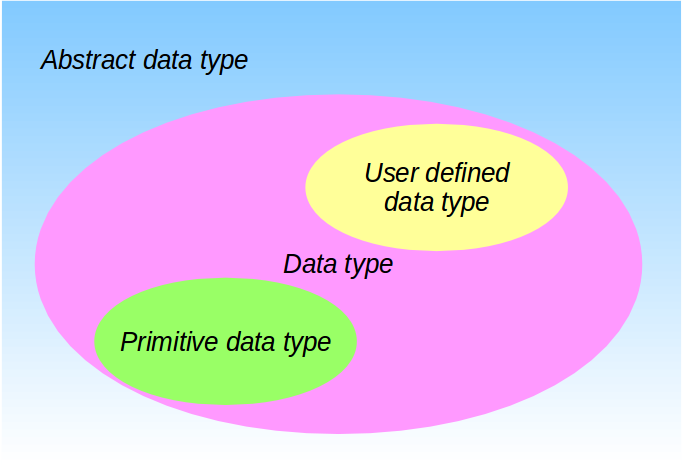
\includegraphics[scale=.5]{pics/datatype.png}
\caption{Hubungan tipe data}
\label{fig:datatype}
\end{figure} 

\section{Prinsip dasar pemrograman}
\label{sec:prinsip}
Prinsip dasar dalam pemrograman tahapan yang harus dilakukan dalam menyelesaikan masalah menggunakan bantuan komputer. Salah satu tahapan dalam pemrograman terstruktur dikenal sebagai \textit{system development life cycle} (SDLC). Tahapan SDLC adalah sebagai berikut.
\begin{enumerate}
\item Analisis masalah: apa yang menjadi masalah, apa saja solusinya, apa dan siapa (pemrograman berorientasi obyek) yang terlibat, tahapan dalam penyelelesaian, indikasi keberhasilan, dll.
\item Membuat \textit{prototype}, umunya dilakukan dalam bentuk \textit{pseduo code} atau diagram alir.
\item Membangun algoritma:
\begin{itemize}
\item merancang \label{sec:rancangan}
\item verifikasi
\item analisis
\item memprogram
\begin{itemize}
\item menguji
\item evaluasi
\item perbaikan (jika perlu)
\item optimasi
\end{itemize}
\item Merawat
\end{itemize}
\end{enumerate}

Dalam merancang algoritma (termasuk juga program yang menerapkan algoritma) seperti disebutkan dalam tahapan ke-\ref{sec:rancangan} dari SDLC, diperlukan tahapan berikut.
\begin{enumerate}
\item Program harus sejalan dengan masalah yang dihadapi, apakah itu prosedur, data maupun struktur datanya.
\item Bekerja baik pada semua kondisi di mana masalah terjadi. Jika ada kondisi di mana solusi yang digunakan tidak dapat mencapai hasil yang diinginkan, kondisi tersebut menjadi pengecualian dan harus disebutkan secara eksplisit.
\item Dokumentasi tentang bagaimana rancangan tersebut dihasilkan (dokumentasi rancangan)
\item Tersusun atas sejumlah modul, fungsi, subrutin. Modularisasi menjadi penting ketika algoritma yang dibangun komplek dan besar. Modularisasi akan memberikan keuntungan dari kemudahan pengembangan.
\item Waktu eksekusi dan ruang penyimpanan yang diperlukan. Kedua hal ini adalah kriteria sebuah algoritma disebut baik. Kebutuhan media penyimpanan yang dimaksud di sini meliputi media yang bersifat \textit{volatile} (\textit{Random Access Memory}/RAM) atau \textit{non-volatile} (\textit{hard disk}). Sementara waktu eksekusi tentu akan berbeda ketika dijalankan di mesin yang berbeda, sehingga ukuran tepatnya adalah jumlah operasi aritmatika dan logika yang dijalankan sebuah algoritma. Nilainya dinotasikan sebagai $\Theta$ atau \textbf{O}. Nilai notasi $\Theta$ untuk beragam struktur data dan algoritmanya diilustasikan pada Gambar \ref{fig:bigOh}\footnote{\url{http://bigocheatsheet.com/}}.
\end{enumerate}

\begin{figure}[H]
\centering
\includegraphics[scale=.45]{../CommonDS.png}
\caption{Perbandingan nilai $\Theta$ sejumlah struktur data dan algoritma}
\label{fig:bigOh}
\end{figure}

Algoritma yang dirancang selanjutnya dianalisis kinerjanya dalam bentuk waktu eksekusi. Selain dipengaruhi oleh mesin di mana algoritma dijalankan, waktu eksekusi juga dipengaruhi oleh masukannya. Sebagai ilustrasi, mengurutkan sejumlah nilai yang telah terurut sebelumnya tentu membutuhkan waktu yang lebih singkat dibanding dengan nilai-nilai yang belum terurut. Waktu eksekusi yang dipengaruhi masukan dapat dikelompokkan dalam 3 kategori.
\begin{enumerate}
\item \textit{Best}: waktu minimum yang diperlukan sebuah algoritma.
\item \textit{Average}: waktu rerata dari eksekusi sebuah algoritma dalam menyelesaikan masalah yang sama dengan masukan yang berbeda. Jika satu masalah memiliki kemungkinan masukan sebanyak $n$, maka waktu rerata adalah rata-rata dari waktu untuk menyelesaikan masalah dengan $n$ masukan tersebut. Jika waktu untuk menyelesaikan algoritma untuk satu jenis masukan adalah $T_i$, maka waktu rerata ($T_{avg}$) dapat diformulasikan dalam persamaan (\ref{eq:tavg}).
\item \textit{Worst}: waktu terburuk sebuah algoritma dalam mengolah satu jenis masukan. 
\end{enumerate}

\begin{equation}
T_{avg}=\frac{\sum_{i=1}^{n}T_i}{n}
\label{eq:tavg}
\end{equation}

Algoritma sendiri dapat didefinisikan sebagai urutan instruksi yang harus diikuti untuk menyelesaikan suatu masalah. Atau dapat juga didefinisikan sebagai prosedur untuk mengubah \textit{input} menjadi \textit{output}. Karakteristik algoritma yang baik adalah sebagai berikut.
\begin{enumerate}
\item Setiap instruksi di dalamnya harus unik dan tepat.
\item Setiap instruksi tidak boleh dijalankan secara berulang tanpa batas.
\item Perulangan tugas yang sama harus dihindari
\item Harus memberikan hasil yang tepat untuk masalah yang dihadapi
\item Efisien dalam menyelesaikan masalah. Faktor efisiensi seperti yang telah disebutkan terdiri dari efisiensi terkait media penyimpanan dan waktu eksekusi.
\end{enumerate} 

\chapter{Bahasa Pemrograman C++}
\section{Pendahuluan}
Bahasa pemrograman \texttt{C++} dipilih dalam diktat ini karena \texttt{C++} secara eksplisit memanfaatkan \textit{pointer} sebagai sarana membangun beragam struktur data. Sementara bahasa pemrograman lain yang lebih modern telah mengemas hal tersebut ke dalam class. Sebagai bahan ajar, \texttt{C++} dinilai lebih mampu memberikan pemahaman tentang merancang dan menerapkan rancangan struktur data ketimbang hanya menggunakan class yang telah terdefinisi dengan baik. Program \ref{hellocpp} memperlihatkan program sederhana \texttt{C++}.

\scriptsize
\begin{lstlisting}[language=c++, numbers=left, numberstyle=\tiny, caption=hello.cpp, showstringspaces=false, label=hellocpp]
#include <iostream>
using namespace std;

int main() {
  cout << "Hello world\n";
  return 0;
}
\end{lstlisting}
\normalsize

Penjelasannya adalah sebagai berikut.
\begin{enumerate}
\item Baris ke-1, merupakan pemanggilan pustaka di mana fungsi-fungsi yang digunakan dalam program diletakkan. Dalam contoh Program \ref{hellocpp}, digunakan fungsi \texttt{cout} yang digunakan untuk menampilkan data ke \textit{standard output} (layar) dan fungsi tersebut didefinisikan di pustaka \texttt{iostream}.
\item Baris ke-2, digunakan untuk menyederhanakan penulisan fungsi. Karena \texttt{C++} adalah bahasa pemrograman berorientasi obyek, setiap fungsi tentu terdefinisi di dalam class tertentu, sehingga pemanggilan terhadap fungsi \texttt{cout} dilakukan apa adanya. Sebaliknya, tanpa deklarasi ini pemanggilan fungsi \texttt{cout} harus dilakukan dengan cara \texttt{std::cout}.
\item Baris ke-4, setiap program berbasis \texttt{C/C++} akan dieksekusi dari fugnsi yang bernama \texttt{main}. Tanpa fungsi ini, program \texttt{C/C++} tidak dapat dieksekusi (proses kompilasi tidak dapat menghasilkan \textit{executable file}).
\item Baris ke-5, digunakan untuk menampilkan teks berupa "Hello World" ke layar.
\item Baris ke-6, digunakan untuk memenuhi syarat berupa \textit{return value} dari fungsi main (Baris ke-4). Biasanya, fungsi yang mengembalikan nilai $0$ disepakati sebagai fungsi yang menjalankan tugas dengan baik. Jika tidak ingin melakukan pengembalian fungsi, maka fungsi \texttt{main} harus diberi tanda \textit{return value} sebagai \texttt{void}.
\item Setiap fungsi dalam \texttt{C/C++} dimulai oleh karakter "\{" dan diakhiri oleh karakter "\}", dan setiap instruksi di akhiri dengan karakter ";".
\item Di terminal, jalankan perintah \texttt{g++ -o hello hello.cpp}, dengan penjelasan.
\begin{itemize}
\item \texttt{g++}: memanggil aplikasi kompilator \texttt{C++}
\item \texttt{-o}: opsi untuk melakukan kompilasi dan \textit{linking} (meski dalam konteks Program \ref{hellocpp} tidak diperlukan) sehingga dihasilkan \textit{executable file}.
\item \texttt{hello}: nama executable file, jika dijalankan di Microsoft Windows dengan bantuan aplikasi MinGW, secara otomatis ditambahkan ekstensi \texttt{.exe}.
\item \texttt{hello.cpp}: kode sumber yang akan dikompilasi
\end{itemize}
\end{enumerate}

\section{IDE}
IDE (\textit{Integrated Development Environment}) adalah aplikasi yang digunakan dalam mengembangkan program. Untuk tujuan mempelajari materi struktur data, sebenarnya nyaris tidak diperlukan IDE. Kita hanya perlu memiliki kompilator \textit{C++} sebagai bahasa pemrograman yang memiliki notasi eksplisit terkait \textit{pointer} (dijelaskan dalam sub bab \ref{sec:pointer}) serta editor teks untuk menulis sejumlah instruksi \texttt{C++}. Untuk pengguna sistem operasi GNU/Linux dalam berbagai variannya, nyaris semua jenis kompilator tersedia secara gratis. Saya sendiri menggunakan editor teks Geany\footnote{\url{https://www.geany.org/}} dengan kompilator \texttt{C++} dari GNU \textit{Project}.

Namun, tidak demikian halnya dengan pengguna sistem Operasi Microsoft Windows. Umumnya, aplikasi di sistem operasi ini dikemas secara terintegrasi, bahkan dengan asumsi kita sedang berhadapan dengan sebuah proyek besar yang butuh cara mengelola proyek (dalam hal ini \textit{software}) yang mumpuni. Padahal, di sisi lain, kita hanya memerlukan editor teks tempat di mana kita menyusun program serta kompilator yang akan membuat program tersebut dapat dijalankan. Beruntung, ada sejumlah aplikasi yang dapat memberikan kita lingkungan pengembangan yang sederhana seperti halnya di sistem operasi GNU/Linux. Misalnya dengan aplikasi MinGW (Minimalist GNU for Windows)\footnote{\url{http://www.mingw.org/}} atau Cygwin\footnote{\url{https://www.cygwin.com/}}. Jangan lupa untuk memasang kompilator \texttt{C++} pada keduanya. Untuk yang masih kesulitan menggunakan aplikasi berbasis perintah baris seperti pada MinGW dan Cygwin, dapat menggunakan aplikasi IDE yang canggih seperti Visual Studio atau NetBeans dengan \textit{plugin} kompilator \texttt{C/C++}.

\section{Tipe data \texttt{pointer} dan \texttt{struct}}
\label{sec:pointer}
Tipe data \textit{pointer} adalah salah satu tipe data yang didefinisikan di \texttt{C/C++}. Tugasnya untuk menunjuk lokasi memori yang menjadi perhatian. Tipe data ini, tidak untuk menyimpan nilai suatu variabel tetapi alamat memori secara fisik di mana suatu nilai disimpan. Meskipun hanya bertugas menunjuk, tetapi tipe datanya harus disesuaikan dengan nilai yang akan ditunjuk. 

Sebagai contoh, untuk mendefinisikan sebuah variabel \textit{integer}, \texttt{C/C++} memiliki sintaks \texttt{int a;}. Untuk membuat sebuah tipe data \textit{pointer} yang akan menunjuk variabel bertipe \textit{integer}, \texttt{C/C++} memiliki sintaks \texttt{int *p;}. Sedangkan untuk membuat \textit{pointer} \texttt{p} menunjuk variabel \texttt{a}, \texttt{C/C++} memilki sintaks \texttt{p=\&a;}. Proses \textit{assignment} tersebut juga dapat dilakukan sekaligus pada saat deklarasi dengan sintaks \texttt{int *p=\&a;}. Intinya, tipe data \textit{pointer} dicirikan dengan karakter "\texttt{*}" di awal variabel dan mengikuti variabel yang ditunjuk. Jika akan digunakan menunjuk vairabel \textit{integer}, maka \textit{pointer} juga harus dideklarasikan sebagai \textit{integer}.

Sebagai contoh, di Gambar \ref{fig:pointer}\footnote{\url{http://stackoverflow.com/questions/4483653/can-you-explain-the-concept-of-the-this-pointer}}, terdapat dua deklarasi variabel. Yang pertama adalah \texttt{val} dengan tipe \textit{integer} yang saat dieksekusi di simpan dalam RAM di alamat \texttt{0xFE}. Sedangkan yang kedua adalah \texttt{*ptr} dengan tipe \texttt{pointer} ke \textit{integer}, tepatnya variabel \texttt{val}. Variabel \texttt{pointer} disimpan di alamat \texttt{0x83} saat diesekusi.

\begin{figure}[H]
\centering
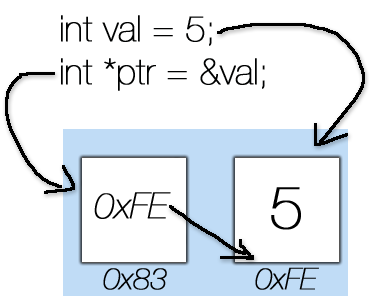
\includegraphics[scale=.5]{pics/pointer.png}
\caption{Ilustrasi penggunaan variabel dengan tipe pointer}
\label{fig:pointer}
\end{figure}

Kemudian, ada tipe data lainnya yang bertugas untuk mengemas sejumlah tipe data yang telah terdefinisi dalam \texttt{C/C++} yang disebut sebagai \texttt{struct}. Tipe data ini memungkinkan kita membuat tipe data baru yang mirip dengan sebuah obyek tanpa fungsi, karena hanya memiliki atribut. Sekali diacu dalam program, maka kita dapat mengakses semua data yang dikemas dalam \texttt{struct}. Program \ref{pointerstruct} mengilustrasikan penggunaan variabel \texttt{pointer} dan \texttt{struct}. Sedangkan Gambar \ref{fig:hasilintro} menunjukkan hasilnya saat dieksekusi. 

Kedua tipe data inilah yang akan banyak digunakan dalam perkuliahan struktur data. Sedangkan yang lainnya hanya pelengkap saja.
\vfill
\scriptsize
\lstinputlisting[language=c++, numbers=left, numberstyle=\tiny, caption=intro.cpp, showstringspaces=false, label=pointerstruct]{coding/intro.cpp}
\normalsize

Penjelasannya adalah sebagai berikut.
\begin{enumerate}
\item Baris ke-4 s/d 7: definisi tipe data baru berupa \texttt{struct data}. Pernyataan \texttt{typedef} di depannya menunjukkan bahwa tipe data \texttt{struct data} memiliki nama alias \texttt{DATA}. Itu sebabnya di baris ke-4 tertulis \texttt{DATA} yang berarti nama alias untuk \texttt{struct data}.
\begin{itemize}
\item Baris ke-5: definisi penyusun pertama \texttt{struct data}, yaitu \texttt{int nilai;}.
\item Baris ke-6: definisi penyusun kedua \texttt{struct data}, yaitu \texttt{struct data *pointer;}. Karena penyusun kedua ini ditugaskan untuk menujukan variabel dengan tipe \texttt{struct data}, maka ia harus didefinisikan dengan tipe yang sama.
\end{itemize}
\item Baris ke-10 dan 11: deklarasi dan \textit{assignment} variabel \textit{integer} dengan nama \texttt{a} dan dengan nilai \texttt{10}.
\item Baris ke-12 dan 13: deklarasi dan \textit{assignment} variabel \texttt{pointer} dengan nama \texttt{*p} dan bernilai \texttt{\&a} (alamat dari variabel \texttt{a} yang disimpan di RAM). 
\item Baris ke-14: deklarasi variabel \texttt{DATA} dengan nama \texttt{x}. Perhatikan kembali cara mendeklarasi variabel di baris ke-10 dan 12.
\item Baris ke-15 dan 16: \textit{assignment} nilai elemen penyusun variabel \texttt{x}, yaitu
\begin{itemize}
\item \texttt{x.nilai=7}
\item \texttt{x.pointer=NULL}: \texttt{pointer} belum menunjuk ke variabel apapun yang bertipe \texttt{DATA}.
\end{itemize}
\item Baris ke-18 s/d 20: menuliskan nilai-nilai yang sebelumnya di-\textit{assign} ke variabel untuk ditampilkan di layar.
\item Baris tanpa penjelasan memiliki penjelasan yang sama dengan penjelasan Program \ref{hellocpp}.
\end{enumerate}

\begin{figure}
\centering
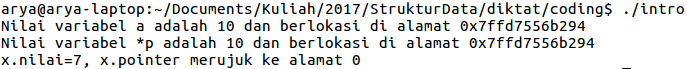
\includegraphics[scale=.5]{pics/hasilintro.png}
\caption{Hasil eksekusi Program \ref{pointerstruct} di terminal}
\label{fig:hasilintro}
\end{figure}

\section{Pemanggilan fungsi}
\texttt{C/C++} memiliki dua skema pemanggilan fungsi, masing-masing adalah pemanggilan fungsi melalui nilai (\textit{calling by value}) dan melalui referensi (\textit{calling by reference}). Skema pertama, argumen fungsi adalah nilai dari yang akan dioperasikan. Jika nilai tersebut terwakili oleh sebuah variabel dalam fungsi asal, maka operasi yang dilakukan tidak akan mempengaruhi nilai pada variabel asalnya. Sebaliknya, pemanggilan fungsi dengan skema kedua memungkinkan perubahan pada nilai variabel asal. Hal ini disebakan karena pemanggilan fungsi dilakukan melalui lokasi absolut RAM di mana nilai tersebut di simpan. Program \ref{calling} akan menunjukkan perbedaannya. Sedangkan Gambar \ref{fig:function} adalah hasil dari eksekusi Program \ref{calling}.

\scriptsize
\lstinputlisting[language=c++, numbers=left, numberstyle=\tiny, caption=function.cpp, showstringspaces=false, label=calling]{coding/function.cpp}
\normalsize

\begin{figure}[H]
\centering
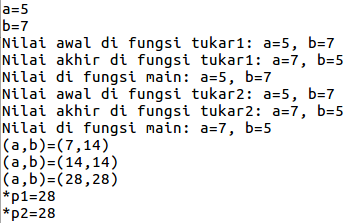
\includegraphics[scale=.5]{pics/hasilfunction.png}
\caption{Hasil eksekusi Program \ref{calling}}
\label{fig:function}.
\end{figure}

Penjelasan dari Program \ref{calling} adalah sebagai berikut.
\begin{enumerate}
\item Baris ke-4 s/d 7: isi dari fungsi yang menerima argumen berupa nilai. Nilai tersebut sejatinya dicopy ke lokasi lain dalam RAM untuk selanjutnya dioperasikan (dalam hal ini akan dikalikan dengan $2$). Hasilnya dikembalikan ke fungsi yang memanggil.
\item Baris ke-9 s/d 12 serta baris ke-14 s/d 17: isi dari fungsi yang menerima argumen berupa alamat dari variabel yang akan dioperasikan. Operasi yang dilakukan fungsi pada variabel akan dilakukan di lokasi yang sama dengan lokasi variabel, sehingga hasilnya akan mengubah nilai asalnya. Kedua fungsi yang sama (\texttt{byReference1} dan \texttt{byReference2}) adalah fungsi dengan pemanggilan melalui referensi dengan notasi yang berbeda.
\item Baris ke-19 s/d 26: isi dari fungsi dengan pemanggilan melalui nilai, tetapi dengan yang berbeda dengan fungsi \texttt{byValue}. Di sini, fungsi hanya menjalankan tugas untuk melakukan pertukaran $2$ nilai yang diberikan.
\item Baris ke-28 s/d 35: isi dari fungsi dengan pemanggilan melalui referensi, tetapi dengan tugas yang berbeda dengan fungsi \texttt{byReference1} dan \texttt{byReference2}. Di sini, fungsi hanya menjalankan tugas untuk melakukan pertukaran $2$ variabel yang diberikan melalui alamatnya.
\item Baris ke-38 s/d 42: deklarasi 2 variabel \textit{integer} serta \textit{assignment} nilai ke kedua variabel tersebut secara langsung melalui \textit{keyboard}.
\item Baris ke-43 dan 44: pemanggilan fungsi \texttt{tukar1} untuk kemudian nilainya ditampilkan kembali untuk melihat pengaruhnya. Maksud yang sama juga dilakukan baris ke-45 dan 46 untuk fungsi \texttt{tukar2}.
\item Baris ke-48: deklarasi variabel \texttt{pointer} dengan nama "\texttt{*p1}" dan "\texttt{*p2}".
\item Baris ke-49 dan 50: pemanggilan fungsi \texttt{byValue} untuk kemudian nilainya di-\textit{assign} ke variabel \texttt{b}. Selanjutnya, nilai variabel \texttt{a} dan \texttt{b} untuk melihat pengaruhnya. 
\item Baris ke-51 dan 52: pemanggilan fungsi \texttt{byReference1} yang menerima argumen berupa lokasi variabel \texttt{a} untuk kemudian nilainya di-\textit{assign} ke variabel \texttt{b}. Selanjutnya, nilai variabel \texttt{a} dan \texttt{b} untuk melihat pengaruhnya. Maksud yang sama juga dilakukan baris ke-54 dan 55 dengan memanggil fungsi \texttt{byReference2}.
\item Sebelumnya, baris ke-53 dilakukan proses \textit{assignment} alamat variabel \texttt{a} ke variabel pointer \texttt{*p1}. Argumen yang diterima fungsi \texttt{byReference1} dan \texttt{byReference2} sama-sama menerima argumen berupa alamat dari variabel \texttt{a}, hanya dengan notasi berbeda. Argumen ke fungsi \texttt{byReference1} adalah alamat variabel \texttt{a} secara langsung, sedangkan argumen ke fungsi \texttt{byReference2} alamat variabel \texttt{a} dilewatkan melalui variabel \texttt{pointer}. Perhatikan kembali Gambar \ref{fig:pointer}.
\item Baris ke-56: menampilkan isi variabel \texttt{a} melalui variabel \texttt{*p1}.
\item Baris ke-57: melakukan \textit{assigment} ke variabel \texttt{*p2} yang isinya adalah \texttt{*p1}. Dalam hal ini, variabel \texttt{*p1} dan \texttt{*p2} menunjuk lokasi yang sama, yaitu lokasi variabel \texttt{a}.
\item Baris ke-58: menampilkan isi variabel \texttt{a} melalui variabel \texttt{*p2}. 
\end{enumerate}

\chapter{\textit{Array dan Linked list}}
\section{\textit{Array}}
Kita dapat membuat variabel yang terdiri dari sejumlah elemen dengan tipe yang sama yang diacu sekaligus. Varibel tersebut, jika selama eksekusi jumlah elemennya tetap disebut sebagai \textit{array}. Sedangkan jika jumlah elemennya berubah disebut sebagai \textit{linked list}. Dengan \textit{linked list}, elemen dari variabel dapat berubah selama eksekusi, baik nilai maupun jumlahnya. Perubahan jumlah elemen dapat terjadi di mana saja, apakah itu di awal, akhir maupun di tengah rangkaian data. Perhatikan Program \ref{array} yang mengilustrasikan kegunaan array dalam \texttt{C++}. Dalam program tersebut, sebuah variabel \textit{array} berelemen 10 bilangan \textit{integer} diisi secara acak untuk kemudian ditampilkan isinya di layar.

\scriptsize
\lstinputlisting[language=c++, numbers=left, numberstyle=\tiny, caption=array.cpp, showstringspaces=false, label=array]{coding/array.cpp}
\normalsize

Penjelasan dari Program \ref{array} adalah sebagai berikut.
\begin{enumerate}
\item Baris ke-2: deklarasi pustaka untuk dapat membuat bilangan \textit{pseudo random} (fungsi \texttt{srand}), sehingga pemanggilan fungsi untuk menghasilkan bilangan random selalu berbeda, dari satu eksekusi ke eksekusi selanjutnya.
\item Baris ke-3: deklarasi pustaka untuk fungsi \texttt{time}.
\item Baris ke-7: deklarasi variabel \textit{array} dengan jumlah elemen 10 bilangan \textit{integer}.
\item Baris ke-9: fungsi yang dapat membuat variabel \texttt{seed} selalu berubah pada setiap eksekusinya karena nilai bergantung pada saat program dieksekusi. Variabel \texttt{seed}\footnote{\url{https://en.wikipedia.org/wiki/Random_seed}} ini adalah variabel yang menentukan bilangan acak yang dihasilkan.
\item Baris ke-10 s/d 12: \textit{looping} untuk mengisi \textit{array} dengan bilangan acak.
\item Baris ke-13 s/d 21: \textit{looping} untuk menampilkan nilai eleman \textit{array}. Dari \textit{looping} ini, terlihat bahwa elemen array dapat diakses langsung melalui nomor index.
\end{enumerate}

\section{\textit{Linked list}}
Untuk \textit{linked list}, sebuah Program \ref{linkedlist} dibuat untuk mensimulasikan penggunaannya. Di awal, \textit{linked list} akan dibuat dengan jumlah 10 elemen. Kemudian, operasi penambahan dan pengurangan elemen dilakukan, baik di awal, maupun akhir elemen \textit{linked list}. Sedangkan Gambar \ref{fig:linkedList} menunjukkan hasil eksekusinya. Program \ref{linkedlist} telah memanfaatkan fitur orientasi obyek dari \texttt{C++}. 

Yang perlu diperhatikan adalah program ini tidak memiliki \textit{destructor}, fungsi yang mendestruksi semua obyek saat program selesai dijalankan. Karena itu, dari sisi penggunaan RAM, program ini terbilang buruk. Hal ini disebabkan karena setiap selesai menjalankan program ini, semua elemen yang pernah dibuat tetap berada di dalam RAM dengan status terisi, meskipun tidak pernah digunakan lagi. Peran yang dijalankan oleh \textit{destructor} disebut sebagai \textit{garbage collector} di pemrograman Java\footnote{\url{http://www.oracle.com/webfolder/technetwork/tutorials/obe/java/gc01/index.html}}. Efisiensi penggunaan media penyimpanan, baik RAM maupun \textit{hardisk}, baik saat disimpan, dijalankan bahkan paska dijalankan yang menjadi kriteria baik tidaknya sebuah program. Hal ini disajikan dalam sub bab \ref{sec:prinsip}.

\scriptsize
\lstinputlisting[language=c++, numbers=left, numberstyle=\tiny, caption=linkedList.cpp, showstringspaces=false, label=linkedlist]{coding/linkedList.cpp}
\normalsize

\begin{figure}[H]
\centering
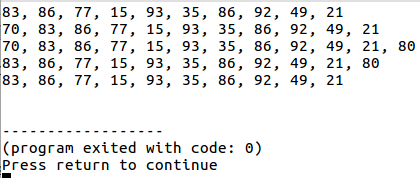
\includegraphics[scale=.5]{pics/hasillinkedlist.png}
\caption{Hasil eksekusi linkedList.cpp}
\label{fig:linkedList}
\end{figure}

Penjelasan dari Program \ref{linkedlist} adalah sebagai berikut.
\begin{enumerate}
\item Baris ke-11 s/d 22: deklarasi class LinkedList. Class ini terdiri dari $2$ atribut dan $6$ fungsi, termasuk \textit{constructor}. Atribut yang terlibat adalah variabel \textit{pointer} yang bertugas menandai elemen pertama (\texttt{awal}) dan terakhir (\texttt{akhir}).
\item Baris ke-24 s/d 45: isi dari fungsi \textit{constructor}. Di sini didefinisikan $10$ elemen pertama dari \textit{linked list}. Pengisian $10$ elemen pertama dilakukan dalam $2$ tahap. Yang pertama, saat elemen pertama diisi, semua pointer \texttt{awal} dan \texttt{akhir} menunjuk pada elemen tersebut (baris ke-34 dan 35). Selain elemen pertama, elemen yang sebelumnya ditunjuk oleh pointer akhir di-\textit{assign} agar menunjuk elemen yang baru (baris ke-41). Sementara pointer akhir di-\textit{assign} untuk menunjuk elemen yang baru.
\item Baris ke-47 s/d 61: isi setiap elemen ditampilkan ke layar dimulai dari elemen pertama.
\item Baris ke-63 s/d 68: elemen baru ditambahkan sebelum elemen pertama, sehingga elemen baru tersebut sekarang menjadi elemen pertama dalam \textit{linked list}.
\item Baris ke-70 s/d 76: elemen baru ditambahkan setelah elemen terakhir, sehingga elemen baru tersebut sekarang menjadi elemen terakhir dalam \textit{linked list}.
\item Baris ke-78 s/d 87: elemen pertama dikeluarkan dari \textit{linked list}.
\item Baris ke-89 s/d 102: elemen terakhir dikeluarkan dari \textit{linked list}.
\item Baris ke-104 s/d 117: isi dari fungsi \texttt{main} berupa pendefinisian obyek \texttt{list}, \texttt{seed} serta pemanggilan terhadap fungsi-fungsi yang telah didefinisikan dalam \textit{class} \texttt{LinkedList}.
\end{enumerate}

\chapter{\textit{Graph}}
\section{Pendahuluan}
\textit{Graph} adalah sarana untuk menyimpan dan menganalisis metadata serta hubungan yang mungkin ada antar data tersebut. \textit{Graph} terdiri dari dua elemen, masing-masing adalah \textbf{vertex} (yang dapat dianalogikan dengan \textit{node}) serta \textbf{edge} yang menghubungkan sejumlah \textbf{vertex}. \textbf{Vertex} tanpa \textbf{edge} sudah dapat disebut sebagai \textit{graph}, tetapi tidak sebaliknya. Gambar \ref{fig:jenisgraph} menunjukkan beberapa jenis \textit{graph}.

\begin{figure}[H]
\centering
\includegraphics[scale=.35]{pics/graph.png}
\caption[Jenis-jenis \textit{graph}]{Jenis-jenis \textit{graph}\cite{adam2001data}}
\label{fig:jenisgraph}
\end{figure}

\textit{Graph} yang terdiri dari sejumlah \textbf{vertex}, dengan atau tanpa \textbf{edge} disebut sebagai \textit{simple graph} (Gambar \ref{fig:jenisgraph} (a)-(d)). Jika setiap \textbf{vertex} dalam \textit{graph} saling terhubung oleh satu \textbf{edge}, \textit{graph} disebut lengkap (\textit{complete graph}). Contohnya ditunjukkan oleh Gambar \ref{fig:jenisgraph} (c). Kemudian, ketika dua \textbf{vertex} berbeda saling terhubung melalui lebih dari satu \textbf{edge}, kondisi tersebut didefinisikan sebagai \textit{multigraph}. Ilustrasinya ditunjukkan oleh Gambar \ref{fig:jenisgraph} (e). Kondisi umum dari multigraph di mana \textbf{vertex} yang sama boleh dihubungkan dengan \textbf{edge} disebut sebagai \textit{pseudograph}. Dengan demikian, akan terjadi \textit{looping} \textbf{vertex} ke dirinya sendiri. Kondisi ini diilustrasikan oleh Gambar \ref{fig:jenisgraph} (f).

\textit{Graph} dengan \textbf{edge} berarah disebut sebagai \textit{directed graph} atau \textit{digraph}. Pada kondisi ini, dua vertex saling terhubung hanya pada arah tertentu. Sebaliknya, jika tidak ada batasan arah pada semua \textbf{edge} dalam \textit{graph}, maka \textit{graph} disebut sebagai \textit{undirected graph}. Jika pada \texttt{edge} di-\textit{assigned} sebuah nilai, maka \textit{graph} disebut dengan \textit{weighted graph}. Bobot dari \textit{graph} bisa bermakna banyak hal, tergantung dalam penerapannya. Program \ref{adjlist} menunjukkan contoh penerapan \textit{graph} dalam \texttt{C++} yang diambil dari laman \url{http://www.sanfoundry.com/cpp-program-implement-adjacency-list/}.

\scriptsize
\lstinputlisting[language=c++, numbers=left, numberstyle=\tiny, caption=adjList.cpp, showstringspaces=false, label=adjlist]{coding/adjList.cpp}
\normalsize

%Sebuah \textit{path}, $v_{1}$ ke $v_{n}$ merupakan rangkaian \textbf{edge}($v_{1}v_{2}$), \textbf{edge}($v_{2}v_{3}$) $\ldots$ \textbf{edge}($v_{n-1}v_{n}$) dan dinotasikan sebagai \textit{path} $v_{1}, v_{2}, v_{3} \ldots v_{n-1}, v_{n}$. Jika $v_{1}=v_{n}$ serta tidak ada \textbf{edge} berulang, maka \textit{path} disebut sebagai sirkuit. Sebuah kondisi khusus dari sirkuit adalah ketika semua \textbf{vertex} yang terlibat dalam \textit{path} tidak ada yang sama.

\chapter{Tugas}
Di kesempatan perkuliahan ini, mahasiswa diminta untuk membuat tulisan di blog dan media lainnya yang dapat diakses secara publik via internet. Tulisannya seputar penerapan struktur data dalam bahasa pemrograman, salah satunya \texttt{C++} yang telah dipelajari. Tulisan harus memiliki aspek berikut.
\begin{enumerate}
\item Skenario tentang struktur data seperti apa yang akan dibuat serta operasi apa saja yang dapat dijalankan pada struktur data tersebut.
\item Ilustrasi (berupa gambar) dari struktur data tersebut.
\item Penerapan program dari struktur data. Program dapat diambil dari kode sumber terbuka yang tersedia di internet. Pastikan menyertakan URL dari program tersebut. Sebagai contoh, mahasiswa dapat mengunjungi laman \url{http://www.sanfoundry.com/cpp-programming-examples-data-structures/} untuk menyelesaikan tugas ini.
\item \textit{Screenshot} hasil eksekusinya.
\end{enumerate} 

\bibliographystyle{apalike}
\bibliography{reference}
\end{document}
